 %aum gaanathipathaye namaha
%srj
\section{\textsc{BinGo} Framework}\label{sec:methodology}
This section, we present the four modules in \tool in details.
As the first step, \tool disassembles the binary and splits it into basic functional units or functions. Then, it constructs the control-flow graph (CFG) for each function, where each CFG is consists of basic-blocks. Later, the constructed CFGs are used to generate the partial traces.
%\ly{when to lift to IR? need to explain this clearly.}
%The definitions of CFG and basic-block are given below:

%\begin{mydef}
%\emph{(\textbf{Basic-block}) }  A sequence of assembly instructions without any jumps or jump targets in the middle, where a jump target starts a block, and a jump ends a block.
%\end{mydef}
%\begin{mydef}
%\emph{(\textbf{Control-flow graph}) } A directed graph, where each node represents a basic-block and edges represent control flow.
%\end{mydef}

\subsection{Partial Trace Extraction} \label{subsec:partial_trace}
%
%In the literature~\cite{pewnycross,lakhotia2013fast,ruttenberg2014identifying}, basic-block is considered as a single building block.
%
%\begin{mydef}
%\emph{(\textbf{Basic-block})}  A sequence of assembly instructions without any jumps or jump targets in the middle, where a jump target starts a block, and a jump ends a block.
%\end{mydef}

%However, it is too restrictive to assume that a function compiled for two different compiler optimization-level (or compiled using two different compilers or in the worst, compiled for two different architectures) will maintain the same basic-block structure. This is vital for cross-architecture and -platform function search.

In \tool, we propose a partial trace based function modeling, which is more flexible in terms of granularity, compared with basic-block centric function modeling techniques~\cite{DBLP:conf/sp/PewnyGGRH15, luo2014semantics}. That is, for each function, we generate partial traces of various lengths, and by varying the length the granularity of single building block is adjusted\footnote{Length of one yields a basic-block centric models, where the basic-block is considered as a single building block.}.

%Partial trace is a sequence of adjacent basic-blocks that lie along a program execution path.
Our partial trace extraction is based on the technique proposed by David \emph{et. al.}~\cite{DBLP:conf/pldi/DavidY14}.
We omit the algorithm and explain the results using one example.
%As discussed in Section~\ref{subsec:bin_pre}, partial traces can be of any length, e.g., partial trace of length 2 is a concatenation of two adjacent basic-blocks along the function CFG.
%, where partial trace of size \textit{k} referred to as \textit{k-tracelet}.
%
%\begin{mydef}
%\emph{\textbf{(\textit{k}-tracelet)}~\cite{david2014tracelet}} k-tracelet is an ordered tuple of k sequences, each representing one of the basic-blocks in a directed acyclic sub-path in the CFG, and containing all of the basic-blocks assembly instructions.
%\end{mydef}
%\note{\textbf{Shall we move the Algorithm below to appendix, as it is not our novelty, just give example in the text?}}
%To be self-contained, we briefly explain the partial trace  extraction algorithm presented in \cite{DBLP:conf/pldi/DavidY14}.
%\note{Algorithm~\ref{algo:k-trace} shows the steps involved in extracting \textit{k}-length partial traces from a CFG. The partial traces are extracted recursively from the nodes in the CFG. To extract all the \textit{k}-length partial traces from a certain node in the CFG, we compute all (\textit{k-1})-length partial traces from any of its \textit{sons}, and use a Cartesian product (\texttt{X}) between the node and the collected partial traces. Algorithm~\ref{algo:k-trace} uses a helper function, \texttt{StripJumps}, which takes a sequence of assembly instructions in which a jump may appear as the last instruction, and returns the sequence without the jump instruction.
%That is, in partial traces, the flow of execution is already determined and hence, all control-flow instructions (e.g., \texttt{jmp}, \texttt{je}, \texttt{jnz}, \ldots) are omitted.}
%\note{\textbf{better to show this example only?}}
Fig.~\ref{fig:example-cfg} depicts a sample CFG of a function and Fig.~\ref{fig:ex-tracelet} presents the extracted partial traces of length 3. From the partial traces it can be see that the original control-flow instructions (\texttt{jnx xxx}, \texttt{jb xxx} and \texttt{jb xxx}) are omitted as the flow of execution is already determined. Note that the feasibility of the flow of execution is not considered when generating the partial traces. However, later in Section~\ref{subsubsec:sou_prun}, we show how the partial traces that are \textit{infeasible} are identified with the help of a constraint solver and removed from our analysis. Here, infeasible partial traces refer to program execution flows that are not possible during any concrete execution.

%\xyx{reachability  is not focus of binary code search}.
%\begin{MyAlgo}[!ht]{-4.9cm} %increase or decrease margin, span across columns
% \DontPrintSemicolon
% \KwData{control-flow graph $CFG$}
% \KwResult{set of k-tracelets $kT$}
% \SetKwFunction{algo}{ExtractTracelets}\SetKwFunction{proc}{Extract}
% \SetKwProg{myalg}{Algorithm}{}{}
% \myalg{\algo{$CFG$}}{
%  $kT \longleftarrow \emptyset$ \tcp*{set of partial traces}
% \ForEach{{\upshape basic-block} b {\upshape in} $CFG$}{
%  %\tcc{write the algo here}
%  $kT \longleftarrow kT \cup Extract(b, k)$\;
%  }
%  \Return ${ kT}$
%  }
%  \setcounter{AlgoLine}{0}
%  \SetKwProg{myproc}{Procedure}{}{}
%  \myproc{\proc{b, k}}{
%  $b_s \longleftarrow StripJumps(b)$\;
%  \eIf{$k == 1$}{
%    \Return $b_s$
%  }{
%   \Return $\bigcup b \times Extract(b^\prime, k-1)$\;
%  }
%  }
% \caption{Partial trace extraction from a fucntion CFG}\label{algo:k-trace}
%\end{MyAlgo}

\begin{figure}[t]
\begin{center}\vspace{-3mm}
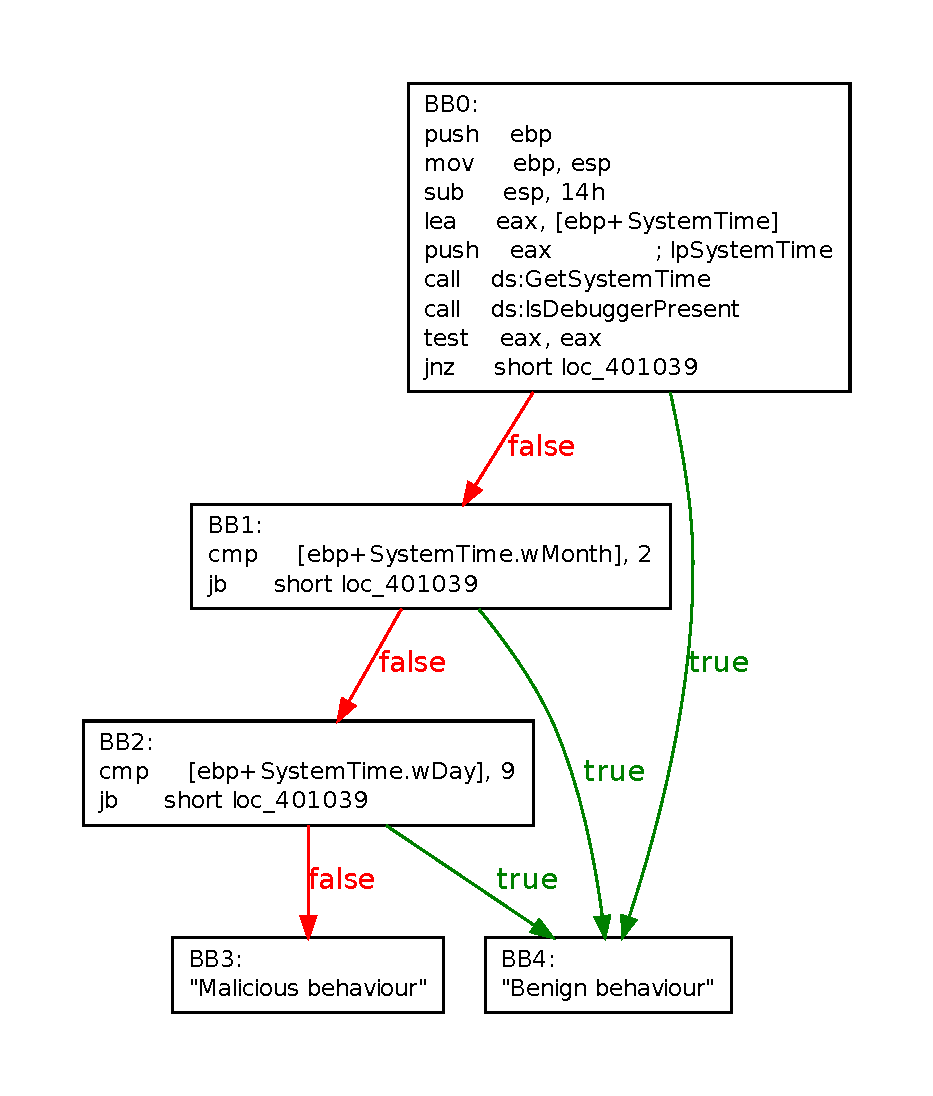
\includegraphics[height=5cm, width=5cm]{srj-figures/srj-toy_malware_cfg.pdf} \vspace{-1mm}
\caption{Sample CFG of a function}
\label{fig:example-cfg} \vspace{-2mm}
\end{center}
\end{figure}


\subsection{Semantic Feature Extraction} \label{subsec:sem_fea_ext}
%\ly{this subsect is very unclear wihout examples}
In this section, we elaborate the feature extraction process from state-based semantic models and behavior models.

\noindent \textbf{Feature extraction from state-based semantic models} \label{subsubsec:sb_sem_mod_fe}
As discussed in Section \ref{subsec:stat_sem}, a set of I/O formulas is extracted from each partial trace, and these formulas capture the relationship between symbolic pre- and post-state values. However, the extracted I/O formulas cannot be directly fed into our machine learning module. Hence, we leverage on the constraint solver to extract features by solving the formulas, where solving refers to finding appropriate values for the input and output vocabularies
%(as discussed in section~\ref{subsec:stat_sem})
such that all the constraints present in the I/O formulas are satisfied. The obtained concrete values for input/output vocabularies constitute  the features of state-based semantic model.
%Here, solving refers to finding appropriate concrete values for symbolic inputs (or input arguments) such that all the constraints are satisfied. Later, using these concrete inputs, the corresponding concrete values are obtained for all output arguments.
For example, consider the following two I/O formulas extracted from a simple example of partial trace:
\begin{eqnarray}
\mathtt{zf^\prime \equiv (edx < 2) \wedge (edx > 0)} \label{eq:IO_1} \\
 \mathtt{ecx^\prime \equiv edx + 4} \label{eq:IO_2}
\end{eqnarray}
For the above I/O formulas, it can be seen that there are two output vocabularies ($\mathtt{zf^\prime}$ and $\mathtt{ecx^\prime}$) and one input vocabulary ($\mathtt{edx}$), where the input vocabulary is common for both I/O formulas. Hence, it is essential to ensure that the concrete value obtained for input vocabulary $\mathtt{edx}$ satisfies the both I/O formulas. That is, for  $\mathtt{zf^\prime}$ to be $\mathtt{true}$, $\mathtt{edx}$ can only take the concrete value $\mathtt{1}$, hence, $\mathtt{ecx^\prime}$ is forced to take the concrete value $\mathtt{5}$. From this example, it is evident that constraint solver is required to find appropriate values for input/output vocabularies, as it takes all the I/O formulas, extracted from a partial trace, into consideration when arriving at the solution. Note  that if there are more than one concrete value for the input/output vocabularies, we  set a limit to $\mathcal{N}$ possible values, where $\mathcal{N}$ is set to 3 in our experiment based on the empirical results reported in~\cite{egele2014blanket}.

In contrast, in the sampling-based feature extraction technique, proposed in the literature~\cite{DBLP:conf/sp/PewnyGGRH15}, each I/O formula is considered independently, where the relationship between the two I/O formulas is ignored (both have the same input vocabulary $\mathtt{edx}$). This approach may lead to inaccurate semantics, especially in case of real-world execution instructions that are executed sequentially. Hence, the relationship between formulas needs to be maintained. However, it is observed that using a constraint solver is costly, compared to sampling-based feature extraction technique.  As feature extraction is an one time task and can be paralleled for binaries that are totally independent of each other, we adopt the constraint solver based approach for its accuracy.


\begin{figure}[t]
\scriptsize
  \begin{subfigure}[b]{0.5\linewidth}
    \centering
   % \includegraphics[width=0.75\linewidth]{srj-figures/srj-hierarchy-2.png}
    \raggedright{\texttt{
    \\
    	push ebp\\
    	mov	ebp, esp\\
   		sub	esp, 14h\\
   		lea eax, [ebp+SysT]\\
   		push eax\\
   		call ds:LibCall1\\
   		call ds:LibCall2\\
   		test eax, eax\\
   		%jnz short loc\_401039\\
   		cmp [ebp+SysT.wMonth],2\\
   		%jb short loc\_401039\\
   		cmp [ebp+SysT.wDay],9\\
   		%jb short loc\_401039
    }}
    \caption{\small{Tracelet $\langle BB0, BB1, BB2\rangle$}}
   \label{fig:traceleta}
    \vspace{1ex}
  \end{subfigure}%%
  \begin{subfigure}[b]{0.5\linewidth}
    \centering
      \raggedright{\texttt{
    \\
    	push ebp\\
    	mov	ebp, esp\\
   		sub	esp, 14h\\
   		lea eax, [ebp+SysT]\\
   		push eax\\
   		call ds:LibCall1\\
   		call ds:LibCall2\\
   		test eax, eax\\
   		%jnz short loc\_401039\\
   		cmp [ebp+SysT.wMonth],2\\
   		%jb short loc\_401039\\
   		benign behaviour
    }}
    \caption{\small{Tracelet $\langle BB0, BB1, BB4\rangle$}}
    \label{fig:traceletb}
    \vspace{1ex}
  \end{subfigure}
  \begin{subfigure}[b]{0.5\linewidth}
    \centering
    \raggedright{\texttt{
    \\
   		cmp [ebp+SysT.wMonth],2\\
   		%jb short loc\_401039\\
   		cmp [ebp+SysT.wDay],9\\
   		%jb short loc\_401039\\
   		benign behaviour
    }}
    \caption{\small{Tracelet $\langle BB1, BB2, BB4\rangle$}}
    \label{fig:traceletc}
  \end{subfigure}%%
  \begin{subfigure}[b]{0.5\linewidth}
    \centering
   \raggedright{\texttt{
    \\
   		cmp [ebp+SysT.wMonth],2\\
   		%jb short loc\_401039\\
   		cmp [ebp+SysT.wDay],9\\
   		%jb short loc\_401039\\
   		malicious behaviour
    }}
    \caption{\small{Tracelet $\langle BB1, BB2, BB3\rangle$}}
    \label{fig:traceletd}
  \end{subfigure}
  \\
  \vspace{-4mm}
  \caption{Tracelets extracted from the CFG shown in Fig.~\ref{fig:example-cfg}\\.\\}
  \label{fig:ex-tracelet}
  \vspace{-4mm}
\end{figure}

%On the other hand, in our approach, we consider the relationship among symbolic expressions. For example consider the following symbolic expressions:
%\begin{itemize}
%\centering
%\itemsep0em
%  \item[] $\mathtt{EAX = EDX + 0x5}$
%  \item[] $\mathtt{ECX = EAX + EBX}$
%\end{itemize}
%
%
%From the above symbolic expressions, it can be seen that both are related via the register $\mathtt{EAX}$. That is, output argument of first symbolic expression (i.e., $\mathtt{EAX}$) is passed as one of the input arguments to the second symbolic expression. Therefore, we can infer that $\mathtt{ECX}$ register depends on $\mathtt{EAX}$, $\mathtt{EBX}$ and $\mathtt{EDX}$ registers. However, this relationship is missing in sample-based feature extraction technique, where for a given value of $\mathtt{EDX}$ register, the value of $\mathtt{EAX}$ register is computed and for a given value of $\mathtt{EAX}$\footnote{Not necessarily the value computed for $\mathtt{EAX}$ register in the first expression is used in the second expression} and $\mathtt{EBX}$ registers, the value of $\mathtt{ECX}$ register is computed. In \tool, the order of symbolic expression irrelevant as the constraint solver accumulate all the symbolic expressions generated from a partial trace before it generates a model that satisfy all the constraints.

\noindent \textbf{Feature extraction from behavior models} \label{subsubsec:abs_sem_mod_fe}
Feature extraction from behavior models is straightforward, where the high-level meanings of the extracted idioms are used as features. For example, if the machine code pattern `\texttt{pop reg}; \texttt{pop reg}; \texttt{pop reg}; \texttt{pop reg};' is observed in the binary code under analysis, using learned idiom patterns and their corresponding high-level meanings (as discussed in Section~\ref{subsubsec:archi_plat_dep}), the code pattern is identified as `\texttt{restore callee-save registers}' and added to features of the behavior model. \idiomDep{Further, using dependency analysis of idioms, related idioms are identified and put together in a tuple. For example, if the two semantic idioms `\texttt{string arithmetic}' and `\texttt{memory manipulation}' are observed to be dependent, they are put together in a tuple as follows: $\langle$\texttt{string arithmetic}, \texttt{memory manipulation}$\rangle$}

%the graph is represented as a sequence of high-level behavioural characteristics. It is important to note that representing related behavioural characteristics as a sequence is completely different from representing all extracted behaviours as a \textit{set}, where in set ordering (i.e., relationship) is ignored. For example, the abstract semantic graph presented in Fig.~\ref{fig:abs} is represented as: $\langle$\textit{data\_movement\_from\_memory, stack\_operation\_store, network\_connection}$\rangle$. Since the abstract semantic graph is a directed acyclic graph, the repeated behaviours are ignored, where they are represented by a single entry in the sequence.
%
%\todo{Do I need to provide example for feature extraction?}

%In contrast to single basic-block based function modelling proposed in the literature, in \tool, we use partial traces of various lengths
%, called \textit{k-tracelet} \cite{david2014tracelet},
%to model the functions.
%Partial trace is a sequence of adjacent basic-blocks that lie along a program execution path. Partial traces can be of any length, for example, partial trace of length 2 (i.e., \textit{2-tracelet}) is a concatenation of two adjacent basic-blocks along the program CFG. A formal definition of \textit{k}-tracelet \cite{david2014tracelet} is given below.

%talk about basic-block terminators?

%\begin{figure}[t]
%	\centering
%	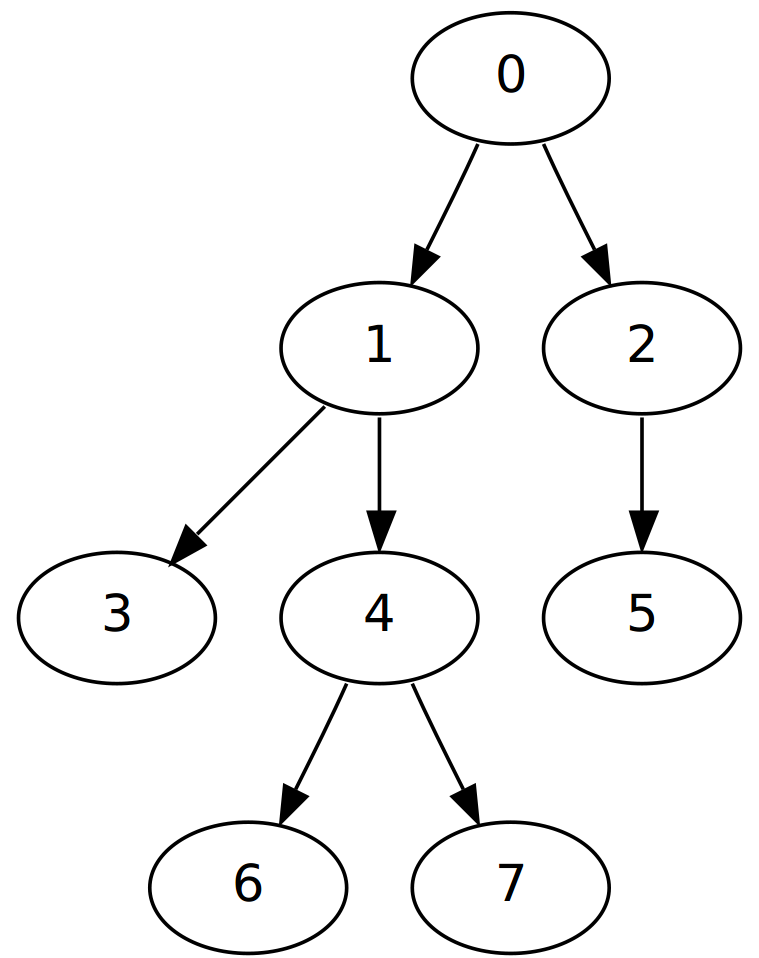
\includegraphics[height=4cm, width=3cm]{srj-figures/tracelet.png}
%	\caption{Control-flow graph (CFG) of a sample fucntion}\label{fig:tracelet}
%\end{figure}
%
%\begin{table}[t]
%\caption{Partial traces generated from a sample fucntion CFG shown in Fig.~\ref{fig:tracelet}}\label{tab:par_tra}
%\begin{center}
%{\scriptsize
%\begin{tabular}{|c|c|}
%  \hline
%  \textbf{$k$} & \textbf{Generated partial traces} \\
%  \hline
%  1 & $\langle 0 \rangle$, $\langle 1 \rangle$, $\langle 2 \rangle$, $\langle 3 \rangle$, $\langle4\rangle$, $\langle 5 \rangle$, $\langle 6 \rangle$, $\langle 7 \rangle$\\
%  \hline
%  2 & $\langle 0,1 \rangle$, $\langle 1,3 \rangle$, $\langle 1,4 \rangle$, $\langle 4,6 \rangle$, $\langle 4,7 \rangle$, $\langle 0,2 \rangle$, $\langle 2,5 \rangle$\\
%  \hline
%  3 & $\langle 0,1,3 \rangle$, $\langle 0,1,4 \rangle$, $\langle 1,4,6 \rangle$, $\langle 1,4,7 \rangle$, $\langle 0,2,5 \rangle$\\
%  \hline
%  \end{tabular}
%}
%\end{center}
%\end{table}

%\begin{table}[!ht]
%\caption{Function models constructed from partial traces shown in Table \ref{tab:par_tra}}\label{tab:func_mod}
%
%\begin{center}
%{\scriptsize
%\begin{tabular}{|m{0.2cm}|m{5.5cm}|m{0.5cm}|}%{|c|c|}
%  \hline
%  \textbf{$n$} & \textbf{Constructed function models} & \textbf{$w_n$}\\
%  \hline
%  1 & $\langle 0 \rangle$, $\langle 1 \rangle$, $\langle 2 \rangle$, $\langle 3 \rangle$, $\langle4\rangle$, $\langle 5 \rangle$, $\langle 6 \rangle$, $\langle 7 \rangle$ & 0.500\\
%  \hline
%  2 & $\langle 0,1 \rangle$, $\langle 1,3 \rangle$, $\langle 1,4 \rangle$, $\langle 4,6 \rangle$, $\langle 4,7 \rangle$, $\langle 0,2 \rangle$, $\langle 2,5 \rangle$ & 0.750\\
%  \hline
%  3 & $\langle 0,1,3 \rangle$, $\langle 0,1,4 \rangle$, $\langle 1,4,6 \rangle$, $\langle 1,4,7 \rangle$, $\langle 0,2,5 \rangle$ & 0.830\\
%  \hline
%    4 & $\langle 0 \rangle$, $\langle 1 \rangle$, $\langle 2 \rangle$, $\langle 3 \rangle$, $\langle4\rangle$, $\langle 5 \rangle$, $\langle 6 \rangle$, $\langle 7 \rangle$, $\langle 0,1 \rangle$, $\langle 1,3 \rangle$, $\langle 1,4 \rangle$, $\langle 4,6 \rangle$, $\langle 4,7 \rangle$, $\langle 0,2 \rangle$, $\langle 2,5 \rangle$ & 0.625\\
%  \hline
%  5 & $\langle 0,1 \rangle$, $\langle 1,3 \rangle$, $\langle 1,4 \rangle$, $\langle 4,6 \rangle$, $\langle 4,7 \rangle$, $\langle 0,2 \rangle$, $\langle 2,5 \rangle$, $\langle 0,1,3 \rangle$, $\langle 0,1,4 \rangle$, $\langle 1,4,6 \rangle$, $\langle 1,4,7 \rangle$, $\langle 0,2,5 \rangle$ & 0.790\\
%  \hline
%  6 & $\langle 0,1,3 \rangle$, $\langle 0,1,4 \rangle$, $\langle 1,4,6 \rangle$, $\langle 1,4,7 \rangle$, $\langle 0,2,5 \rangle$, $\langle 0 \rangle$, $\langle 1 \rangle$, $\langle 2 \rangle$, $\langle 3 \rangle$, $\langle4\rangle$, $\langle 5 \rangle$, $\langle 6 \rangle$, $\langle 7 \rangle$ & 0.665\\
%  \hline
%  7 & $\langle 0,1 \rangle$, $\langle 1,3 \rangle$, $\langle 1,4 \rangle$, $\langle 4,6 \rangle$, $\langle 4,7 \rangle$, $\langle 0,2 \rangle$, $\langle 2,5 \rangle$, $\langle 0 \rangle$, $\langle 1 \rangle$, $\langle 2 \rangle$, $\langle 3 \rangle$, $\langle4\rangle$, $\langle 5 \rangle$, $\langle 6 \rangle$, $\langle 7 \rangle$, $\langle 0,1,3 \rangle$, $\langle 0,1,4 \rangle$, $\langle 1,4,6 \rangle$, $\langle 1,4,7 \rangle$, $\langle 0,2,5 \rangle$ & 0.693\\
%  \hline
%
%  \end{tabular}
%}
%\vspace{-4mm}
%\end{center}
%\end{table}

\subsection{Function Model Generation} \label{subsec:fun_mod}
Compiler optimizations and/or differences in environments often lead to changes in the basic-block structure. Thus, basic-block centric function modeling is not preferred~\cite{DBLP:conf/sp/PewnyGGRH15,luo2014semantics}.  For example, given a search query that consists of a single basic block, we may miss the similar function in the target binary pool due to the structural difference, where the semantically similar target function can be of several basic-blocks and the similarity between the query function and each of the basic-blocks in the candidate target function can be below the pre-defined threshold value. This is a common observation that arises due to differences in compiler optimization and the compiler types that lead to basic-block splitting (or merging) and function inclining (or outlining). Hence, in \tool, as discussed in Section~\ref{subsec:partial_trace}, we use k-length partial traces to model the functions. The key advantage of using partial trace, over other techniques~\cite{DBLP:conf/sp/PewnyGGRH15,luo2014semantics}, lies in its resilience to the structural changes incurred by the aforementioned compiler optimization techniques, which otherwise might fail the similarity search.
%That is, partial traces generated at various lengths from the search query function are matched against the partial traces of different lengths generated from the functions in the target function pool.
However, in the step of generating partial traces,  the generated partial traces need to be valid or feasible in real-world executions. To this end, we propose a \textit{pruning} technique to remove partial traces that are \textit{infeasible} in practise.
 %\note{absolutely}

\subsubsection{Pruning of Partial Traces} \label{subsubsec:sou_prun}

%\note{THEOREM 2. Given a template T , an oracle, and any nsyn ,
%nver , if T is sufficient for abstracting ��, then the procedure
%DInputVal(, T, nsyn , nver ) returns a function C semantically
%equivalent to .
%A useful corollary is that, if the procedure DInputVal returns ��In-
%sufficient Template�� for any nsyn , nver , then the template T is in-
%deed insufficient for abstracting ��. However, this theorem is weaker
%than Theorem 1 as it does not guarantee that the procedure returns
%��Insufficient Template�� whenever the template is insufficient.
%Just like procedure ExhaustVal, DInputVal provides a satis- \\
%}


\tool is a static analysis based tool and hence, it is relatively difficult (or impossible) to identify all the partial traces that are infeasible in practise. In \tool, we prune the obvious infeasible partial traces with the help of a constraint solver. That is, given a partial trace, we extract the set of I/O formulas, as explained in Section~\ref{subsec:stat_sem}, and try to generate a model that satisfied all the constraints present in the I/O formulas (i.e., able to generate appropriate concrete values for input/out vocabularies), if such model is not available then that partial trace is considered infeasible.
%and pass them to the solver, which will try to solve the constraints and generate a model that satisfies them all. If the solver fails to generate a model, we label that partial trace as infeasible and prune it from the analysis.
Some  partial traces, for which the solver is able to generate models, might be infeasible during real world execution, as the feasibility of their paths depends on various factors, such as global variables, values in the heap and other dynamic data, that are beyond the scope of static analysis.
Infeasible path elimination is a difficult task even in dynamic analysis. Comparing to the static analysis solutions proposed in the literature \cite{DBLP:conf/pldi/DavidY14,pewny2014leveraging,luo2014semantics,DBLP:conf/sp/PewnyGGRH15}, this work makes an attempt to reduce the search candidates using pruning technique.

%\note{On the other hand, if a solver is unable to generate a model for a partial trace then it is indeed infeasible as there are no real values that can be substituted for the symbolic variables (i.e., symbolic registers, flags and memory locations) such that all the constraints are solved. Even though we are unable to prune all the infeasible partial traces, comparing to the static analysis solutions proposed in the literature \cite{david2014tracelet,pewny2014leveraging,pewnycross}, we are heading towards the right direction of eliminating infeasible paths in analysis.}

Even with the infeasible partial traces pruned, it is still difficult to compare the signature function against those functions in the target binary pool. Thus, a systematic way of performing the similarity matching among partial traces is desired. Specifically, the question ``what length of partial traces in the search query needs to be matched with what length of partial traces in the target function?'' still persists.
%To this end, we propose a simple function modelling technique to represent each function using partial traces of various lengths.

\subsubsection{Function Modeling} \label{subsubsec:fun_mod}

\begin{figure}[t]
% \begin{minipage}{.5\textwidth}
%\lstinputlisting[language=C]{srj-figures/srj-openssl_code.c}
%   (a)
%\end{minipage}
  \centering
  %\includegraphics[width = 7cm,height=4.5cm]{srj-figures/srj-func_model_match.pdf} %original_version
   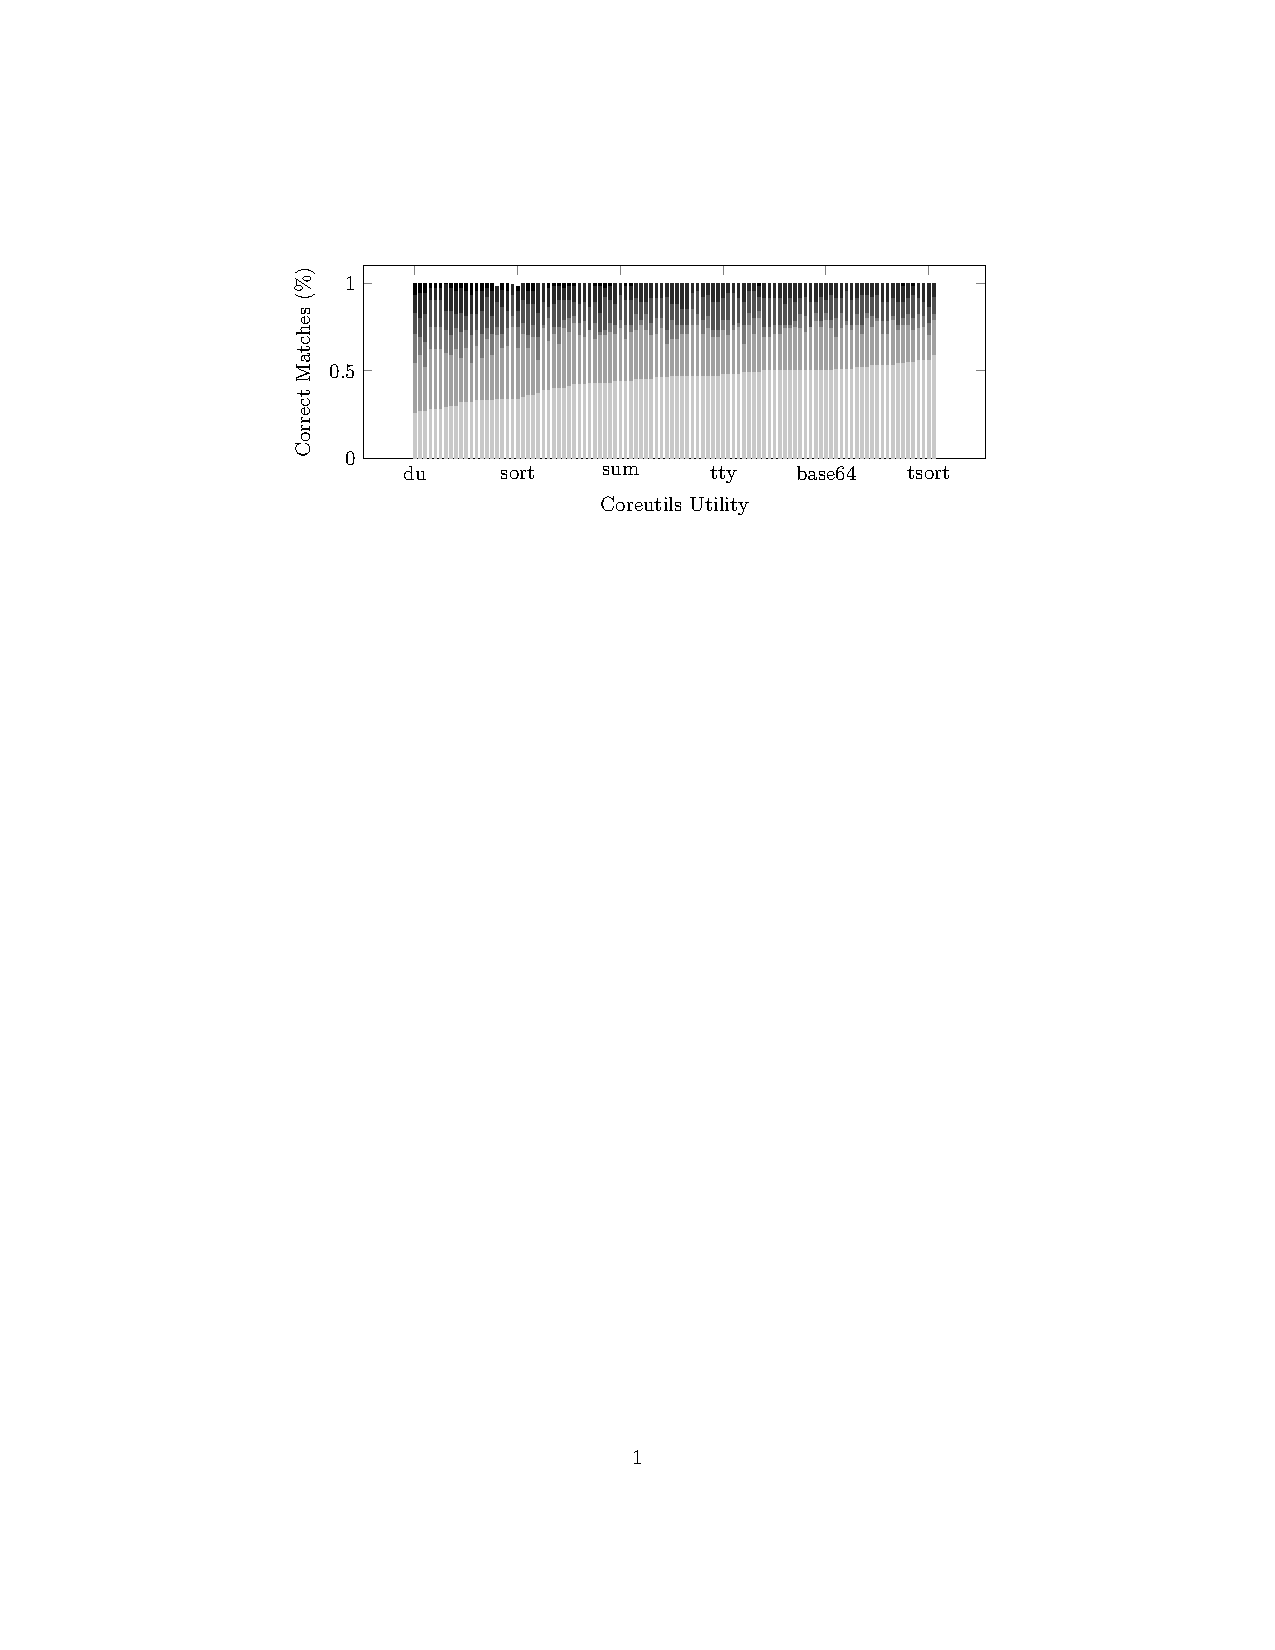
\includegraphics[width = 7cm,height=4.5cm]{srj-figures/the_graph.pdf} %the_graph
  \caption{This depicts the signature and target functions, where the lines indicate the matched partial traces.} \label{fig:func_mod}
  %\vspace{-2mm}
\end{figure}


It is understood that partial traces need to be organized in a systematic way to effectively compare two different functions.
As the signature and the target functions are shown in Fig.~\ref{fig:func_mod} (a) and (b) respectively, it can be seen that these two functions are matched as follows: the partial traces $\mathtt{ \langle 4,7,9 \rangle}$,  $\mathtt{ \langle 3,6,8 \rangle}$,  $\mathtt{ \langle 1 \rangle}$,  $\mathtt{ \langle 5 \rangle}$,   $\mathtt{ \langle 2 \rangle}$  in the signature function  are matched with the partial traces  $\mathtt{ \langle d \rangle}$,   $\mathtt{ \langle c \rangle}$,   $\mathtt{ \langle z,a \rangle}$,  $\mathtt{ \langle e,f,g \rangle}$,  $\mathtt{\langle b \rangle}$  in the target function, respectively.
%The set of partial traces (i.e., partial traces of lengths 1, 2 and 3) extracted from these two functions are shown in Fig.~\ref{fig:func_mod} (c) and (d),
Hence, we can say those combination of partial traces \textit{precisely model} the underlying functions. Here, precise model of a function (called \emph{precise function model}) refers to a combination of partial traces that can cover every single basic-block in the CFG without any overlap. That is, a basic-block should not be covered by more than one partial trace. Precise  models for the functions shown in Fig.~\ref{fig:func_mod} is as follows:
\begin{itemize}
\centering
\itemsep0em
  \item[] $\mathtt{Signature \; Function:  \lbrace \langle 1 \rangle,  \langle 2 \rangle, \langle 5 \rangle, \langle 4,7,9 \rangle, \langle 3,6,8 \rangle \rbrace}$
   \item[] $\mathtt{Target \; Function: \lbrace \langle c \rangle,  \langle b \rangle, \langle d \rangle, \langle z,a \rangle, \langle e,f,g \rangle \rbrace}$
\end{itemize}

However, it is challenging to identify all possible combinations of partial traces that can precisely model a function. Further, it is also not very scalable for larger functions, which are very common in real-world binaries. Hence, in \tool, to improve the scalability, we limit the function models to a fixed number by relaxing the precision. That is, instead of ensuring that the partial traces do not overlap, we construct function models (called \emph{relaxed function models}), where none of the basic-blocks are missed, however, there can be overlapping of partial traces. In the rest of the sections, for simplicity, relaxed function model is also refereed to as function model and is formally defined as follows:
%\st{That is, in a relaxed function model, a single basic-block can be covered by multiple partial traces, however, non of the basic-blocks are missed.}

\begin{mydef}
\emph{\textbf{(Function model)}} It is a unique combination of partial traces. Given $\mathtt{N}$ different lengths of partial traces, generated from a function, in total, $\mathtt{2^N-1}$ function models are constructed for that function.
\end{mydef}

%For example, partial traces of three different lengths (i.e., $k=1,2,3$), generated from the function CFG shown in Fig.~\ref{fig:tracelet}) is presented in Table~\ref{tab:par_tra}. From the table, it can be seen that there are, in total, 20 partial traces are generated from the function.

%From the partial traces presented in Table~\ref{tab:par_tra} (assuming all the partial traces are feasible), 7 (i.e., $2^3-1$) function models are constructed and they are listed in Table~\ref{tab:func_mod}. For example, from the table, it can be seen that function model 1 consists of partial traces of length 1, model 4 consists of partial traces of lengths 1 and 2, and model 7 consists of all partial traces.
%
%One might argue that function model 7 alone would be sufficient as it contains all the partial traces. However, these are not precise function models, instead, relax function models with huge redundancy. We observe that  more than required partial traces reduce the similarity score due to high noise to signal ratio. Hence, it is essential to match all function models in signature function with all function models in the target functions to identify the optimal function model for signature and target functions (discussed in the next section).


%may lead to higher false positive rate. This is due to the fact that, in \tool, as explained in section \ref{subsubsec:sb_sem_mod_fe}, a constraint solver is used to solve the symbolic expressions. Given the complexity of constraints there can be more than one possible assignments to symbolic arguments that can satisfy all the constraints. That is, given the constraints are too trivial to solve, input arguments present in two different symbolic expressions might be assigned the same values, which, in this case, considered false positive.
%
%For example, consider the following two `toy' constraints obtain from two different partial traces:
%\begin{eqnarray}
%\mathtt{0x10 = eax+ebx} \label{eq:cons_1} \\
%\mathtt{0x10 = ecx-edx} \label{eq:cons_2}
%\end{eqnarray}
%From the Equations \ref{eq:cons_1} and \ref{eq:cons_2}, we can see that they are quite trivial and the symbolic registers $\mathtt{\langle eax,ebx\rangle}$ and $\mathtt{\langle ecx,edx\rangle}$ can possibly have too many satisfying assignments. Interestingly, the default satisfying model generated by Z3 solver for Equation \ref{eq:cons_1} is $\mathtt{eax=0x10}$ and $\mathtt{ebx=0x00}$, and for Equation \ref{eq:cons_2} is $\mathtt{ecx=0x10}$ and $\mathtt{edx=0x00}$. Therefore, given the values assigned to the symbolic registers, both the partial traces have the same effect on the program state and hence, considered similar, which is false. It is noted that, in \tool, we abstract away the register name to account for various register names used across multiple architectures. Thus, the assignments $\mathtt{eax=0x10}$ and $\mathtt{ecx=0x10}$ are considered same, where the value $\mathtt{0x10}$ is assigned to a register.
%
%To address the aforementioned issue, in function model matching (discussed in Section~\ref{subsec:fun_mod_mat}), we encourage matching between function models that are composed of larger partial traces by assigning different weights to each model. That is, function model matching between larger partial traces has higher weights than the smaller partial traces. This is based on the observation that larger partial traces tend to have complex constraints, which limits the number of possible satisfying assignment to symbolic variables and hence, reduce the false positive rate. The weights for function models are assigned using Equation~\ref{eq:wei_ass}.
%\begin{eqnarray}
%\mathtt{w_n=\frac{1}{\vert K_n \vert}\sum_{\substack{\mathtt{k} \in \mathtt{K_n}}}\left(1-\frac{1}{2*k} \right)} \label{eq:wei_ass}
%\end{eqnarray}
%Here, $\mathtt{w_n}$ refers to the weight assigned to function model $n$ and $\mathtt{K_n}$ refers to the set of different partial trace types (in terms of length) present in function model $n$. For example, the weight for function model 7 ($\mathtt{w_7}$) is determined as follows: there are three types of partial traces (i.e., $\mathtt{K_7={1,2,3}}$) and the individual weights for partial trace lengths 1, 2 and 3 are $\mathtt{0.50, 0,75}$ and $\mathtt{0.83}$, respectively, finally, the combined weight is calculated to be $\mathtt{0.693}$ ($=\mathtt{(0.50+0.75+0.83)/3}$).

\subsection{Function Model Matching} \label{subsec:fun_mod_mat}

One of the key advantages of function model is that it enables \textit{n-to-m}, \textit{1-to-n}, \textit{n-to-1} and \textit{1-to-1} matches across the signature\footnote{Signature function refers to the search query function in hand.} and target functions\footnote{Similarly, target functions refer to functions in the target binary pool against which the signature function is matched.}, eliminating the impact of optimizations and differences of compilers.

\begin{description}
  \item[\textit{n-to-m}] Partial traces of the length $n (\in\mathbb Z_{> 1})$ generated from the signature function are matched against the partial traces of the length $m (\in\mathbb Z_{> 1})$ generated from target function. For example, from Fig.~\ref{fig:func_mod}, partial trace matches: $\langle 3,6,8\rangle$ and  $\langle d,g\rangle$.
  \item[\textit{1-to-n}] Each basic-block (i.e., partial trace of the length 1) in the signature function is matched against the partial traces of $n (\in\mathbb Z_{> 1})$ generated from target function. From Fig.~\ref{fig:func_mod}, partial trace matches: $\langle 1\rangle$ and $\langle a,b\rangle$.
  \item[\textit{n-to-1}] Partial traces of the length $n (\in\mathbb Z_{> 1})$ generated from the signature function are matched against each basic-block in the target function. From Fig.~\ref{fig:func_mod}, partial trace matches:  $\langle 4,7,9 \rangle$ and $\langle e \rangle$.
  \item[\textit{1-to-1}] Each basic-block in the signature function is matched against each basic-block in the target function. It is also known as pairwise comparison of basic-blocks. From Fig.~\ref{fig:func_mod}, partial trace matches:  $\langle 2\rangle$ and $\langle c\rangle$.
\end{description}

Among the four types of matching, \textit{1-to-n} matching addresses the issue of basic-block splitting --- a single basic-block in the signature function is split into several smaller basic-blocks in the target function. Similarly, \textit{n-to-1} matching addresses the basic-block merging problem. On the other hand, \textit{n-to-m} mapping is generally preferred when the signature (target) function is part of a huge target (signature) function and appropriately selected values for $n$ and $m$ will maximize the function similarity. Finally, if none of the aforementioned matching techniques work, we resort to \textit{1-to-1} matching to compare the basic-block similarity in a pairwise way, which is similar to those basic-block centric comparison approaches~\cite{DBLP:conf/sp/PewnyGGRH15,luo2014semantics}.

In \tool, the function model matching is not fixed, where, for a given signature function, the searching algorithm will try all possible function models and pick the best one that maximizes the signature-target function similarity. In contrast, the techniques proposed in the literature do not have the flexibility to try out all possible matchings. For example, in tracelet-based modeling \cite{DBLP:conf/pldi/DavidY14}, the authors recommended that the tracelet size should be larger (e.g., $k>2$), for both signature and target functions, hence, only \textit{n-to-m} matching is performed, in fact, it is \textit{n-to-n} matching as they consider the same tracelet size for both signature and target functions. Further, in~\cite{DBLP:conf/sp/PewnyGGRH15} and~\cite{luo2014semantics}, pairwise comparison of basic-blocks (i.e., \textit{1-to-1} matching) is performed as an initial step to identify potential target functions, which inherently assumes that the program structure is maintained across signature and target functions and at least one basic-block in the target function resembles a basic-block in the signature function.

%\subsubsection{Similarity measure} \label{subsubsec:sim_mea}
%During function model matching process, the similarity between different function models (e.g., $f_a$ and $f_b$) is measured using Jaccard distance:
%\begin{equation}
%\begin{aligned}
%Jaccard(f_a, f_b) = \frac{\vert f_a \cap f_b \vert}{\vert f_a \cup f_b \vert}
%\end{aligned}
%\end{equation}

%\subsubsection{Example - \note{\textbf{REMOVE this section}}} \label{subsubsec:exp}
%
%\begin{figure}
%\centering
%\noindent
%\begin{minipage}{.11\textwidth}
%\begin{lstlisting}[caption=BB1,frame=tlrb]{Name}
%push ebp
%mov ebp, esp
%\end{lstlisting}
%\end{minipage}\hfill
%\begin{minipage}{.11\textwidth}
%\begin{lstlisting}[caption=BB2,frame=tlrb]{Name}
%pop ebx
%mov ecx, ebx
%\end{lstlisting}
%\end{minipage}\hfill
%\begin{minipage}{.15\textwidth}
%\begin{lstlisting}[caption=sym. expr for BB1 (partial trace with length 1),frame=tlrb]{Name}
%ESP' = ESP - 0x4
%[ESP - 0x4] = EBP
%EBP = ESP - 0x4
%\end{lstlisting}
%\end{minipage}\hfill
%
%\begin{minipage}{.15\textwidth}
%\begin{lstlisting}[caption=sym. expr for BB2 (partial trace with length 1),frame=tlrb]{Name}
%ESP' = ESP + 0x4
%EBX = [ESP]
%ECX = [ESP]
%\end{lstlisting}
%\end{minipage}\hfill
%\begin{minipage}{.20\textwidth}
%\begin{lstlisting}[caption=sym. expr for both BBs combined (partial trace with length 2),frame=tlrb]{Name}
%ESP' = ESP - 0x4 + 0x4
%[ESP - 0x4] = EBP
%EBP = ESP - 0x4
%EBX = [ESP - 0x4]
%ECX = [ESP - 0x4]
%\end{lstlisting}
%\end{minipage}
%\caption{Sample basic-blocks and their corresponding symbolic expressions at two different granularity levels} \label{fig:sym_expr_granu}
%\end{figure}
%
%Figure \ref{fig:sym_expr_granu} depicts the sample basic-blocks (assuming they are adjacent and lie along the execution path in a function CFG) and the corresponding symbolic expressions extracted for partial traces of the length $1$ and $2$, denoted as PT-1 and PT-2, respectively. From the example, it can be seen that \texttt{ESP}, \texttt{EBX} and \texttt{ECX} registers hold different values in PT-2 model (see listing 5) compare to PT-1 model (see listing 3 and 4). That is, when two basic-blocks are merged, the extracted semantic features change considerably, which in return, will have an adversarial effect in vulnerability signature matching process. Thus, it is vital to extract semantic features at a suitable granularity level such that the vulnerabilities are not missed.

\subsection{Locality Sensitive Hashing} \label{subsec:lsh} %\note{replace this with simple feature hasing technique, if no time, leave as it is.. not very important}
In \tool, we leverage on Locality-sensitive Hashing (LSH) technique to perform the function matching more efficiently and in a scalable manner. Locality-sensitive hashing is an algorithm for searching similar items in large and high dimensional dataset \cite{leskovec2014mining} based on the assumption that, if two items are similar, the hashed value of the two items will remain similar. In \tool, we use MinHashing~\cite{broder1997resemblance} technique to hash the extracted features and generate hash signature for each function model. To this end, we use 1000 (i.e., $n=1000$) hash functions to generate the signature, which leads to an error of 3.16\%. The similarity between two function model is given by this equation:
\begin{equation}
\begin{aligned}
 sim(mh_a, mh_b) = \frac{\vert mh_a[i]=mh_b[i ]\vert}{n}
\end{aligned}
\end{equation}
where the jaccard similarity between two function models is approximated by MinHash similarity between the two models.


%\subsection{Post-processing} \label{subsubsec:post-proc}
%One challenge in matching smaller functions is that the number of semantic features that can be extracted is very limited, which may lead to a high false positive rate. This is one of the key limitations for static analysis based on function modelling techniques~\cite{david2014tracelet,pewnycross}. For example, in \cite{david2014tracelet}, all the functions need to satisfy the minimum basic-blocks requirement, where functions with less than 100 basic-blocks are ignored from the analysis. We find this requirement is very restrictive in real-world applications. For example, in \texttt{msvcrt.dll}, the \texttt{strlen} function has only 14 basic-blocks, and also the same function has only 20 basic-blocks in \texttt{libc}.
%
%Hence, in \tool, we add a post-processing step that removes the limitation of matching (or searching) small functions. In post-processing process, we clear up the search results by removing the false positives. To this end, we leverage on clustering technique to identify false positives. That is, from the initial search results (i.e., before post-processing), we extract all the function names that appear within top 500 ranks\footnote{If the search results contain less than 500 functions, we take the entire results.}. Extracting function names at the binary level is possible as our target function pool contains only open-source binaries and in general, function name indicates the high-level functionality of a functions \note{cite ref}. Later, from the extracted function names, treating them as some random strings, we construct n-grams models of various lengths. In \tool, we construct tri-gram ($n=3$) and four-gram ($n=4$) models from each function name and use them as features to do the clustering. For example, features extracted from the function name \texttt{strlen} is as follows:
%\begin{eqnarray}
%\mathtt{F_3 = \lbrace str,trl,rle,len\rbrace}  \\
%\mathtt{F_4 = \lbrace strl,trle,rlen\rbrace}
%\end{eqnarray}
%
%Here, $\mathtt{F_3}$ and $\mathtt{F_4}$ refer to tri-gram and four-gram features, respectively. Once the clustering is done, we remove the clusters with only 1 element (or function name), where a cluster with 1 (or very few) elements is considered `outlier' in machine learning terminology. It is important to note that, using this technique, we can only remove completely unrelated functions (or outliers) from the search results and cannot remove the functions that appear similar to the search query at the function name-level (e.g., \texttt{strlen} vs. \texttt{strcpy}). Even though, post-processing module can only remove outliers, we find this very useful as it completely removes the unwanted results and keep only the related ones (at least at the function name-level). We remark that it is possible incorporate more domain specific heuristics in this module to further improve the accuracy, e.g., .
